\documentclass[11pt]{article}

\usepackage[margin=1in]{geometry}
\usepackage[T1]{fontenc}
\usepackage{lmodern}
\usepackage{microtype}
\usepackage{amsmath,amssymb,amsthm,mathtools}
\usepackage{mathrsfs}
\usepackage[dvipsnames]{xcolor}
\usepackage[most]{tcolorbox}
\usepackage{graphicx}
\graphicspath{{figures/}{notes/figures/}}
\usepackage{tikz}
\usetikzlibrary{decorations.markings,patterns}
\usepackage{pgfplots}
\pgfplotsset{compat=1.17}
\usepackage{enumitem}
\usepackage{tocloft}
\usepackage[hidelinks]{hyperref}

\definecolor{courseblue}{HTML}{1F4E79}
\definecolor{lightblue}{HTML}{EAF2F8}
\definecolor{lightgreen}{HTML}{EAF7EA}
\definecolor{lightpink}{HTML}{FCE8EF}
\definecolor{lightyellow}{HTML}{FFF8D6}
\definecolor{warningyellow}{HTML}{D6A000}
\definecolor{exercisebg}{HTML}{FDEAEA}
\definecolor{exerciseframe}{HTML}{B54040}
\definecolor{examplebg}{HTML}{F4FAFE}
\definecolor{exampleframe}{HTML}{85C1E9}
\definecolor{darkgray}{HTML}{333333}
\definecolor{lightorange}{HTML}{FDEBD8}
\definecolor{orangeframe}{HTML}{E08A3C}
\definecolor{remarkbg}{HTML}{F3EEFB}
\definecolor{remarkframe}{HTML}{9B7FC9}
\definecolor{cayleyred}{HTML}{C0392B}
\definecolor{cayleygreen}{HTML}{1E8449}
\definecolor{cayleyblue}{HTML}{1F5FA0}
\definecolor{cayleyorange}{HTML}{D35400}
\definecolor{cayleypurple}{HTML}{7D3C98}
\definecolor{cayleyteal}{HTML}{117A65}

\setlength{\parindent}{0pt}
\setlength{\parskip}{0.45em}
\setlist[itemize]{topsep=0.25em,itemsep=0.15em}
\renewcommand{\cftsecleader}{\cftdotfill{\cftdotsep}}
\renewcommand{\cftsubsecleader}{\cftdotfill{\cftdotsep}}

\theoremstyle{plain}
\newtheorem{theorem}{Theorem}[section]
\newtheorem{proposition}[theorem]{Proposition}
\newtheorem{lemma}[theorem]{Lemma}
\newtheorem{corollary}[theorem]{Corollary}
\theoremstyle{definition}
\newtheorem{definition}[theorem]{Definition}
\newtheorem{example}[theorem]{Example}
\newtheorem{exercise}[theorem]{Exercise}
\newtheoremstyle{boldremark}
  {3pt}{3pt}{\normalfont}{}{\bfseries}{.}{.5em}
  {\thmname{#1}\thmnumber{ #2}\thmnote{ (#3)}}
\theoremstyle{boldremark}
\newtheorem*{remark}{Remark}
\theoremstyle{remark}
\newtheorem*{fact}{Fact}
\newtheorem*{warning}{Warning}

\tcolorboxenvironment{definition}{
  enhanced,
  unbreakable,
  colback=lightgreen,
  colframe=ForestGreen,
  boxrule=0.7pt,
  arc=2pt,
  left=6pt,
  right=6pt,
  top=5pt,
  bottom=5pt
}

\tcolorboxenvironment{remark}{
  enhanced,
  colback=remarkbg,
  colframe=remarkframe,
  before upper={\setlength{\parskip}{0.5em}},
  boxrule=0.7pt,
  arc=2pt,
  left=6pt,
  right=6pt,
  top=5pt,
  bottom=5pt
}

\tcolorboxenvironment{warning}{
  enhanced,
  colback=lightyellow,
  colframe=warningyellow,
  boxrule=0.7pt,
  arc=2pt,
  left=6pt,
  right=6pt,
  top=5pt,
  bottom=5pt
}

\tcolorboxenvironment{exercise}{
  enhanced,
  colback=exercisebg,
  colframe=exerciseframe,
  boxrule=1pt,
  arc=2pt,
  left=6pt,
  right=6pt,
  top=5pt,
  bottom=5pt
}

\tcolorboxenvironment{example}{
  enhanced,
  colback=examplebg,
  colframe=exampleframe,
  boxrule=0.7pt,
  arc=2pt,
  left=6pt,
  right=6pt,
  top=5pt,
  bottom=5pt
}

\numberwithin{equation}{section}

\newcommand{\be}{\begin{eqnarray}}
\newcommand{\ee}{\end{eqnarray}}
\newcommand{\C}{\mathbb{C}}
\newcommand{\R}{\mathbb{R}}
\newcommand{\N}{\mathbb{N}}
\newcommand{\Z}{\mathbb{Z}}
\DeclareMathOperator{\Log}{Log}
\DeclareMathOperator{\Arg}{Arg}

\DeclareMathOperator{\Hol}{\mathcal{H}\mathrm{ol}}
\DeclareMathOperator{\Real}{Re}
\DeclareMathOperator{\Imag}{Im}
\newcommand{\A}{\mathcal{A}}
\newcommand{\CT}{\C[[T]]}
\newcommand{\CLT}{\C((T))}
\tcbset{breakable}
% Compact spacing around diagrams; keep the main text at 11pt.
\newenvironment{lecturefigure}
 {\par\addvspace{0.25em}\begingroup\setlength{\parskip}{0pt}\centering}
 {\par\endgroup\addvspace{0.25em}}
\begin{document}

\begin{center}
  \colorbox{lightblue}{%
    \begin{minipage}{0.94\textwidth}
      \vspace{0.55em}
      \begin{tabular*}{\textwidth}{@{\extracolsep{\fill}}lr}
        {\color{courseblue}\bfseries\LARGE Lecture 31} &
        {\color{courseblue}\bfseries\LARGE MATH 411}\\[0.35em]
        \textbf{Fall 2026} & \textbf{Date: Nov 30, 2026}\\
        & \textbf{Instructor: Manish Patnaik}
      \end{tabular*}
      \vspace{0.45em}
    \end{minipage}}
\end{center}

\setcounter{tocdepth}{1}
\tableofcontents
\vspace{0.45em}

% Moved from Lecture 30, Section 4 (handwritten Lecture 29, Nov. 29, pp. 4--6).
\section{Gaussian summation and theta inversion}

Recall from Lecture~30 that if $f\in\mathcal F_a$ for some $a>0$, then its
Fourier transform $\widehat f(\xi)=\int_{-\infty}^{\infty}f(x)e^{-2\pi ix\xi}\,dx$
satisfies the Poisson summation formula
\[
 \sum_{n\in\Z} f(n) = \sum_{n\in\Z}\widehat f(n).
\]
We now apply Poisson summation to the Gaussian function. Recall from
Lecture~14 (Theorem~2.1) and Lecture~29 that
\[
 g(x) = e^{-\pi x^2}
 \qquad\Longrightarrow\qquad
 \widehat g(\xi) = \int_{-\infty}^{\infty} e^{-\pi x^2}e^{-2\pi i x\xi}\,dx
 = e^{-\pi\xi^2}.
\]
Consider the scaled and shifted variant, depending on parameters $t>0$ and
$a\in\R$:
\[
 f(x) = e^{-\pi t(x+a)^2}.
\]
First, note that $f\in\mathcal F_c$ for every $c>0$: indeed,
$f(z)=e^{-\pi t(z+a)^2}$ is entire, and for $z=x+iy$ with $|y|<c$ we have
$\Real\bigl((z+a)^2\bigr)=(x+a)^2-y^2\geq (x+a)^2-c^2$, hence
\[
 |f(x+iy)| = e^{-\pi t((x+a)^2-y^2)} \leq e^{\pi t c^2} e^{-\pi t(x+a)^2},
\]
which decays much faster than $(1+x^2)^{-1}$ as $|x|\to\infty$.

Next, we compute $\widehat f(\xi)$ by a change of variables. Set
$u=\sqrt{t}\,(x+a)$, so $x=t^{-1/2}u-a$ and $dx=t^{-1/2}\,du$:
\begin{align*}
 \widehat f(\xi)
 &= \int_{-\infty}^{\infty} e^{-\pi t(x+a)^2}e^{-2\pi i x\xi}\,dx \\
 &= t^{-1/2}\int_{-\infty}^{\infty}
    e^{-\pi u^2}e^{-2\pi i(t^{-1/2}u-a)\xi}\,du \\
 &= t^{-1/2} e^{2\pi i a\xi}
    \int_{-\infty}^{\infty} e^{-\pi u^2}e^{-2\pi i u(\xi/\sqrt t)}\,du \\
 &= t^{-1/2} e^{-\pi\xi^2/t} e^{2\pi i a\xi}.
\end{align*}
Applying Poisson summation to $f$ immediately gives the following identity.

\begin{proposition}[Shifted Gaussian summation]\label{prop:gaussian-poisson}
For every $t>0$ and $a\in\R$,
\begin{equation}\label{eq:gaussian-poisson}
 \sum_{n=-\infty}^{\infty} e^{-\pi t(n+a)^2}
 = t^{-1/2}\sum_{n=-\infty}^{\infty} e^{-\pi n^2/t} e^{2\pi i n a}.
\end{equation}
\end{proposition}

\begin{definition}[The theta function]
For $t>0$, the \emph{theta function} is defined by
\[
 \Theta(t) = \sum_{n\in\Z} e^{-\pi t n^2}
           = 1 + 2\sum_{n=1}^{\infty} e^{-\pi t n^2}.
\]
Equivalently, separating the $n=0$ term gives
\[
 \Theta(t) - 1 = \sum_{\substack{n\in\Z \\ n\neq 0}} e^{-\pi n^2 t}
               = 2\sum_{n=1}^{\infty} e^{-\pi n^2 t}.
\]
\end{definition}

Setting $a=0$ in Proposition~\ref{prop:gaussian-poisson} yields the
fundamental transformation law of $\Theta$.

\begin{corollary}[Theta inversion formula]\label{cor:theta-inversion}
For every $t>0$,
\begin{equation}\label{eq:theta-inversion}
 \boxed{\displaystyle
  \Theta(t) = t^{-1/2}\,\Theta\!\left(\frac{1}{t}\right).}
\end{equation}
\end{corollary}

The theta inversion formula relates the behavior of $\Theta(t)$ near $t=0$
(where the defining series converges very slowly) to its behavior for large
$t$ (where the series converges rapidly to $1$). This yields two essential
estimates.

\begin{proposition}[Basic consequences of $\Theta$-inversion]\label{prop:theta-bounds}
There exists a constant $C>0$ such that:
\begin{enumerate}[label=\textup{(\arabic*)}]
 \item $\Theta(t) \leq C t^{-1/2}$ for all $0<t\leq 1$ (in particular,
       $\Theta(t)\leq C t^{-1/2}$ as $t\to 0^+$);
 \item $|\Theta(t)-1| \leq C e^{-\pi t}$ for all $t\geq 1$.
\end{enumerate}
\end{proposition}

\begin{proof}
We first prove (2). For $t\geq 1$, separating the $n=0$ term and pairing
$n$ with $-n$ gives
\[
 |\Theta(t)-1| = \Theta(t)-1 = 2\sum_{n=1}^{\infty} e^{-\pi n^2 t}.
\]
Since $n^2\geq n$ for every integer $n\geq 1$ and $t>0$, we have
$e^{-\pi n^2 t}\leq e^{-\pi n t}$. Comparing with a geometric series gives
\[
 |\Theta(t)-1|
 \leq 2\sum_{n=1}^{\infty} e^{-\pi n t}
 = 2\cdot\frac{e^{-\pi t}}{1-e^{-\pi t}}.
\]
Because $t\geq 1$, we have $e^{-\pi t}\leq e^{-\pi}<1$, so
$1-e^{-\pi t}\geq 1-e^{-\pi}>0$. Setting
\[
 B = \frac{2}{1-e^{-\pi}} > 0,
\]
we have $\frac{2}{1-e^{-\pi t}}\leq B$ for all $t\geq 1$, and hence
\[
 |\Theta(t)-1| \leq B e^{-\pi t} \qquad (t\geq 1).
\]

Now we prove (1). Since each summand $e^{-\pi t n^2}$ is continuous and
decreasing in $t>0$, the function $\Theta(t)$ is continuous on $(0,\infty)$
and bounded for $t\geq 1$; indeed, from (2) we have
\[
 0 < \Theta(t) \leq \Theta(1) \leq 1 + B e^{-\pi} \qquad (t\geq 1).
\]
For $0<t\leq 1$, we have $1/t\geq 1$, so the theta inversion formula
\eqref{eq:theta-inversion} yields
\[
 \Theta(t) = t^{-1/2}\Theta\!\left(\frac{1}{t}\right)
 \leq \Theta(1)\,t^{-1/2}.
\]
Since $\Theta(1)\leq 1+\frac{2e^{-\pi}}{1-e^{-\pi}}=\frac{1+e^{-\pi}}{1-e^{-\pi}}<\frac{2}{1-e^{-\pi}}=B$,
the constant $C=B$ works for both (1) and (2).
\end{proof}

\begin{lecturefigure}
\begin{minipage}{\linewidth}\centering
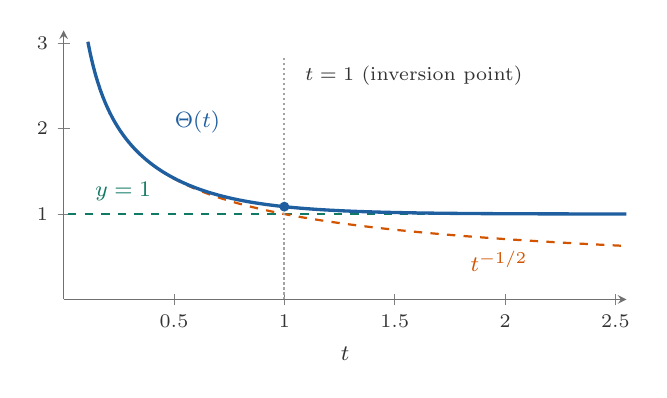
\begin{tikzpicture}[>=stealth]
 \begin{axis}[
   width=0.72\linewidth,
   height=5.0cm,
   axis lines=left,
   axis line style={darkgray!70},
   xmin=0, xmax=2.55,
   ymin=0, ymax=3.15,
   xtick={0.5, 1, 1.5, 2, 2.5},
   ytick={1, 2, 3},
   tick label style={font=\scriptsize, text=darkgray},
   xlabel={$t$},
   xlabel style={font=\footnotesize, text=darkgray},
   ylabel={},
   clip=true
  ]
  % Asymptote y = 1 (t -> infinity)
  \addplot[cayleyteal, dashed, thick, domain=0.02:2.55, samples=2] {1};
  % Asymptote y = t^{-1/2} (t -> 0+)
  \addplot[cayleyorange, dashed, thick, domain=0.11:2.55, samples=160] {1/sqrt(x)};
  % Exact Theta(t) using theta inversion for t < 1
  \addplot[cayleyblue, very thick, domain=0.11:2.55, samples=220] {
    x >= 1
      ? (1 + 2*exp(-3.1415927*x) + 2*exp(-4*3.1415927*x))
      : ((1 + 2*exp(-3.1415927/x) + 2*exp(-4*3.1415927/x))/sqrt(x))
  };
  % Symmetry line t = 1
  \draw[darkgray!45, densely dotted, thick] (axis cs:1,0) -- (axis cs:1,2.85);
  \fill[cayleyblue] (axis cs:1,1.08643) circle (1.8pt);
  % Labels
  \node[font=\footnotesize, text=cayleyblue, anchor=west] at (axis cs:0.46,2.08) {$\Theta(t)$};
  \node[font=\footnotesize, text=cayleyorange, anchor=north west] at (axis cs:1.80,0.68) {$t^{-1/2}$};
  \node[font=\footnotesize, text=cayleyteal, anchor=south west] at (axis cs:0.10,1.04) {$y=1$};
  \node[font=\scriptsize, text=darkgray, anchor=west] at (axis cs:1.05,2.62) {$t=1$ (inversion point)};
 \end{axis}
\end{tikzpicture}

\vspace{0.15em}
{\small Behavior of $\Theta(t)$: for $t\geq 1$, $\Theta(t)$ approaches $1$
exponentially fast ($\Theta(t)-1=O(e^{-\pi t})$); by theta inversion
$\Theta(t)=t^{-1/2}\Theta(1/t)$, as $t\to 0^+$ it closely tracks $t^{-1/2}$.}
\end{minipage}
\end{lecturefigure}


% Source: handwritten Lecture 30, Nov. 30, pp. 1--2.
\section{The Riemann zeta function and the Mellin transform}

Our next major goal is to use the theta function $\Theta(t)$ and its
inversion formula to study the \emph{Riemann zeta function} $\zeta(s)$.
The bridge between $\Theta$ and $\zeta$ is the following integral identity,
which we will prove once we have established the basic analytic properties
of $\zeta(s)$ and the \emph{Gamma function} $\Gamma(s)$.

\begin{theorem}[Mellin transform representation]\label{thm:mellin-zeta}
If $\Real s > 1$, then
\begin{equation}\label{eq:mellin-zeta}
 \boxed{\displaystyle
  \pi^{-s/2}\,\Gamma\!\left(\frac{s}{2}\right)\zeta(s)
  = \frac{1}{2}\int_0^{\infty} u^{s/2-1}\bigl(\Theta(u)-1\bigr)\,du.}
\end{equation}
\end{theorem}

The right-hand side of \eqref{eq:mellin-zeta} is an example of a
\emph{Mellin transform}: for a function $g$ on $(0,\infty)$, its Mellin
transform is $\int_0^{\infty} u^{z-1}g(u)\,du = \int_0^{\infty} g(u)\,u^z\,\frac{du}{u}$.
Notice that the two estimates in Proposition~\ref{prop:theta-bounds} ensure
that the integral on the right of \eqref{eq:mellin-zeta} converges for
$\Real s > 1$: near $u=0$, the integrand is $O(u^{\Real(s)/2-3/2})$, which
is integrable when $\Real(s)/2 - 3/2 > -1$ (i.e., $\Real s > 1$); near
$u=\infty$, $\Theta(u)-1 = O(e^{-\pi u})$ decays exponentially.

Before proving Theorem~\ref{thm:mellin-zeta}, let us carefully define
$\zeta(s)$ and $\Gamma(s)$.

\begin{definition}[The Riemann zeta function]
For $s\in\C$ with $\Real s > 1$, the \emph{Riemann zeta function} is
defined by the Dirichlet series
\[
 \zeta(s) = \sum_{n=1}^{\infty}\frac{1}{n^s},
\]
where $n^s = e^{s\log n}$ (using the real logarithm $\log n$ for $n\geq 1$).
\end{definition}

\begin{proposition}[Convergence and holomorphicity of $\zeta(s)$]\label{prop:zeta-hol}
The series $\sum_{n=1}^{\infty} n^{-s}$ converges absolutely for
$\Real s > 1$ (and diverges at $s=1$), and defines a holomorphic function
$\zeta(s)$ on the half-plane $\{s\in\C:\Real s > 1\}$.
\end{proposition}

\begin{proof}
Write $s=\sigma+it$ with $\sigma,t\in\R$. Then
\[
 n^s = e^{(\sigma+it)\log n} = e^{\sigma\log n}e^{it\log n} = n^{\sigma}n^{it}.
\]
Since $|e^{it\log n}|=1$, we obtain $|n^s|=n^{\sigma}$, and therefore
\[
 \sum_{n=1}^{\infty}\frac{1}{|n^s|} = \sum_{n=1}^{\infty}\frac{1}{n^{\sigma}}.
\]
By the $p$-series test, this series converges for every $\sigma > 1$ and
diverges at $\sigma = 1$ (the harmonic series).

To see that $\zeta$ is holomorphic on $\{s\in\C:\Real s > 1\}$, fix any
$\sigma_0 > 1$. On the closed half-plane $\{s\in\C:\Real s \geq \sigma_0\}$,
each term satisfies $|n^{-s}|=n^{-\sigma}\leq n^{-\sigma_0}$, and
$\sum_{n=1}^{\infty} n^{-\sigma_0}<\infty$. By the Weierstrass $M$-test,
the partial sums $\sum_{n=1}^{N} n^{-s}$ converge uniformly on
$\{\Real s \geq \sigma_0\}$, and hence uniformly on every compact subset of
$\{\Real s > 1\}$. Since each term $s\mapsto n^{-s}=e^{-s\log n}$ is entire, uniform
convergence on closed rectangles together with Morera's theorem
(Lecture~21) and Proposition~2.1 of Lecture~20 shows that the limit
$\zeta(s)$ is holomorphic on $\{\Real s > 1\}$.
\end{proof}

Over the next two lectures we will establish two fundamental facts about
$\zeta(s)$:
\begin{enumerate}[label=\textup{(\arabic*)}]
 \item \textbf{Analytic continuation:} $\zeta(s)$, initially defined only
       on the half-plane $\{\Real s > 1\}$, can be analytically continued to
       all of $\C$ as a meromorphic function (with only a single simple pole
       at $s=1$).
 \item \textbf{Functional equation and symmetry:} The continued function
       satisfies a symmetry across the \emph{critical line}
       $\Real s = \tfrac12$, inside the \emph{critical strip}
       $0\leq\Real s\leq 1$, relating its values at $s$ and $1-s$.
\end{enumerate}

\begin{lecturefigure}
\begin{minipage}{\linewidth}\centering
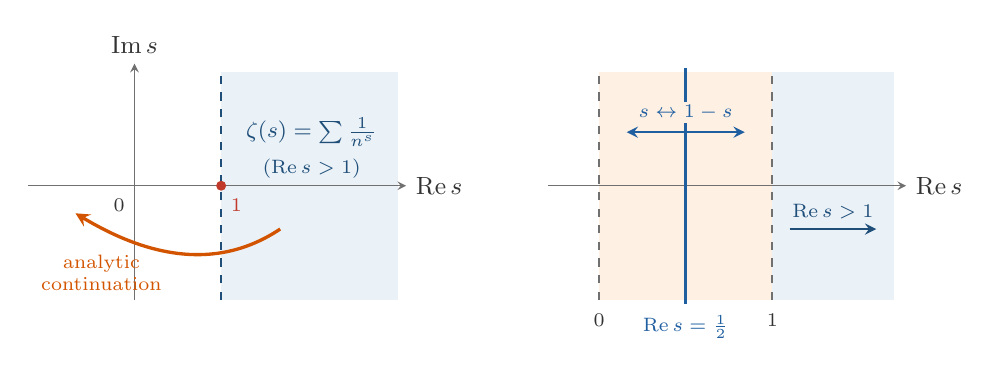
\begin{tikzpicture}[>=stealth,font=\small]
 % Left panel: Analytic continuation from Re s > 1 to C
 \begin{scope}
  \fill[lightblue] (1.1,-1.45) rectangle (3.35,1.45);
  \draw[darkgray!70,->] (-1.35,0) -- (3.45,0) node[right,text=darkgray] {$\Real s$};
  \draw[darkgray!70,->] (0,-1.45) -- (0,1.55) node[above,text=darkgray] {$\Imag s$};
  \draw[courseblue,dashed,thick] (1.1,-1.45) -- (1.1,1.45);
  \fill[cayleyred] (1.1,0) circle (1.8pt);
  \node[below left,font=\scriptsize,text=darkgray] at (0,-0.04) {$0$};
  \node[below right,font=\scriptsize,text=cayleyred] at (1.1,-0.04) {$1$};
  \node[text=courseblue,font=\footnotesize] at (2.25,0.68) {$\zeta(s)=\sum\frac{1}{n^s}$};
  \node[text=courseblue,font=\scriptsize] at (2.25,0.22) {$(\Real s>1)$};
  \draw[->,cayleyorange,very thick]
   (1.85,-0.55) .. controls (1.1,-1.05) and (0.25,-0.95) .. (-0.75,-0.35);
  \node[text=cayleyorange,font=\scriptsize,align=center] at (-0.42,-1.10) {analytic\\continuation};
 \end{scope}

 % Right panel: Critical strip 0 <= Re s <= 1 and critical line Re s = 1/2
 \begin{scope}[xshift=5.9cm]
  \fill[lightorange!70] (0,-1.45) rectangle (2.2,1.45);
  \fill[lightblue] (2.2,-1.45) rectangle (3.75,1.45);
  \draw[darkgray!70,->] (-0.65,0) -- (3.90,0) node[right,text=darkgray] {$\Real s$};
  \draw[darkgray!70,dashed,thick] (0,-1.45) -- (0,1.45);
  \draw[darkgray!70,dashed,thick] (2.2,-1.45) -- (2.2,1.45);
  \draw[cayleyblue,very thick] (1.1,-1.50) -- (1.1,1.50);
  \node[below,font=\scriptsize,text=darkgray] at (0,-1.50) {$0$};
  \node[below,font=\scriptsize,text=darkgray] at (2.2,-1.50) {$1$};
  \node[below,font=\scriptsize,text=cayleyblue] at (1.1,-1.52) {$\Real s=\tfrac12$};
  \draw[<->,cayleyblue,thick] (0.35,0.68) -- (1.85,0.68);
  \node[above,yshift=2pt,font=\scriptsize,text=cayleyblue,fill=lightorange!70,inner sep=1.2pt] at (1.1,0.72) {$s\leftrightarrow 1-s$};
  \draw[->,courseblue,thick] (2.42,-0.55) -- (3.52,-0.55)
   node[midway,above,font=\scriptsize,text=courseblue] {$\Real s>1$};
 \end{scope}
\end{tikzpicture}

\vspace{0.15em}
{\small Left: $\zeta(s)$ is defined initially by $\sum_{n=1}^{\infty}n^{-s}$
on $\{\Real s>1\}$ and extended meromorphically to $\C$ (with a pole at $s=1$).
Right: the critical strip $0\leq\Real s\leq 1$ and its axis of symmetry, the
critical line $\Real s=\tfrac12$.}
\end{minipage}
\end{lecturefigure}


% Source: handwritten Lecture 30, Nov. 30, pp. 2--4.
\section{Holomorphicity of parameter-dependent integrals}

Before turning to $\zeta(s)$, we investigate the Gamma function
$\Gamma(s)=\int_0^{\infty} e^{-t}t^{s-1}\,dt$ ($\Real s > 0$). Our first
task is to verify that this improper integral defines a holomorphic
function of $s$. More generally, we ask: \emph{when does an integral
depending on a complex parameter define a holomorphic function?}

\begin{definition}[Absolute and uniform integrability]
\leavevmode
\begin{enumerate}[label=\textup{(\arabic*)}]
 \item A continuous function $f:[0,\infty)\to\C$ is \emph{absolutely
       integrable} if
       \[
        \int_0^{\infty} |f(t)|\,dt
        = \lim_{B\to\infty}\int_0^{B} |f(t)|\,dt < \infty.
       \]
 \item Let $U\subseteq\C$ be open and let $f:[0,\infty)\times U\to\C$ be
       continuous. Given a subset $K\subseteq U$, we say that the integral
       $\int_0^{\infty} f(t,z)\,dt$ is \emph{uniformly integrable} (or
       \emph{uniformly convergent}) for $z\in K$ if for every $\varepsilon>0$
       there exists $B_0>0$ (independent of $z\in K$) such that for all
       $B_2 > B_1 > B_0$ and all $z\in K$,
       \[
        \left|\int_{B_1}^{B_2} f(t,z)\,dt\right| < \varepsilon.
       \]
\end{enumerate}
More generally, if $I\subseteq\R$ is any interval (possibly open or
unbounded at one or both ends, such as $I=(0,\infty)$), we say that
$\int_I f(t,z)\,dt$ is \emph{uniformly integrable} for $z\in K$ if for
every $\varepsilon>0$ there exists a compact subinterval $J_0\subset I$
such that $\bigl|\int_J f(t,z)\,dt\bigr|<\varepsilon$ for every compact
subinterval $J\subset I\setminus J_0$ and all $z\in K$ (equivalently, for
every increasing exhaustion of $I$ by compact subintervals
$I_1\subseteq I_2\subseteq\cdots\subset I$ with $\bigcup_{n=1}^{\infty}I_n=I$,
the truncated integrals $F_n(z)=\int_{I_n} f(t,z)\,dt$ converge uniformly
for $z\in K$).
\end{definition}

\begin{lemma}[Holomorphicity of parameter-dependent integrals]\label{lem:hol-integral}
Let $I\subseteq\R$ be an interval (possibly open or unbounded), let
$U\subseteq\C$ be open, and let $f:I\times U\to\C$ be continuous. Assume:
\begin{enumerate}[label=\textup{(\roman*)}]
 \item for each compact subset $K\subseteq U$, the integral
       $\int_I f(t,z)\,dt$ is uniformly integrable for $z\in K$;
 \item for each fixed $t\in I$, the function $z\mapsto f(t,z)$ is
       holomorphic on $U$.
\end{enumerate}
Then the function
\[
 F(z) = \int_I f(t,z)\,dt
\]
is holomorphic on $U$, and its derivative is given by differentiating under
the integral sign:
\begin{equation}\label{eq:diff-under-int}
 F'(z) = \int_I \frac{\partial}{\partial z} f(t,z)\,dt.
\end{equation}
\end{lemma}

\begin{proof}
Fix a point $z_0\in U$ and choose $r>0$ small enough that the closed disc
$\overline{D}=\overline{D(z_0,r)}$ lies inside $U$. Let $\gamma=\partial D$
be its boundary circle oriented counterclockwise.

\begin{lecturefigure}
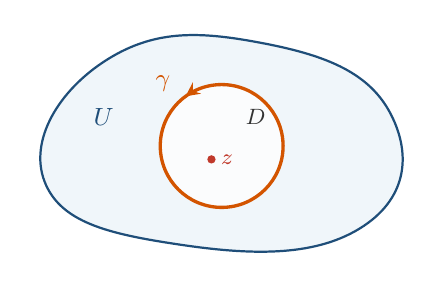
\begin{tikzpicture}[>=stealth,font=\small,
 midarrow/.style={postaction={decorate},decoration={markings,mark=at position .35 with {\arrow{>}}}}]
 % Domain U
 \fill[lightblue!70] plot[smooth cycle,tension=0.8] coordinates
  {(-2.1,-0.4) (-1.3,1.15) (0.7,1.35) (2.3,0.45) (1.9,-1.0) (-0.4,-1.2)};
 \draw[courseblue,thick] plot[smooth cycle,tension=0.8] coordinates
  {(-2.1,-0.4) (-1.3,1.15) (0.7,1.35) (2.3,0.45) (1.9,-1.0) (-0.4,-1.2)};
 \node[courseblue] at (-1.35,0.42) {$U$};
 % Disc D with boundary gamma
 \fill[white,fill opacity=0.75] (0.15,0.05) circle (0.78);
 \draw[cayleyorange,very thick,midarrow] (0.15,0.05) circle (0.78);
 \node[cayleyorange,above left] at (-0.38,0.62) {$\gamma$};
 \node[darkgray,font=\footnotesize] at (0.58,0.42) {$D$};
 \fill[cayleyred] (0.02,-0.12) circle (1.5pt) node[right,font=\footnotesize,text=cayleyred] {$z$};
\end{tikzpicture}

{\small Applying Cauchy's integral formula on $\gamma=\partial D\subset U$
to each integrand $f(t,\cdot)$.}
\end{lecturefigure}

\textbf{Step 1: Reduction to compact intervals $I_n$.}
Choose an increasing sequence of compact subintervals
$I_1\subseteq I_2\subseteq\cdots\subset I$ exhausting $I$ (for instance,
$I_n=[1/n,n]$ when $I=(0,\infty)$, or $I_n=[0,n]$ when $I=[0,\infty)$), and
define
\[
 F_n(z) = \int_{I_n} f(t,z)\,dt.
\]
For each $t\in I_n$ and every $z\in D$, hypothesis~(ii) and Cauchy's
integral formula give
\[
 f(t,z) = \frac{1}{2\pi i}\int_{\gamma}\frac{f(t,\zeta)}{\zeta-z}\,d\zeta.
\]
Integrating both sides over $I_n$, we obtain
\[
 F_n(z) = \frac{1}{2\pi i}\int_{I_n}
          \left(\int_{\gamma}\frac{f(t,\zeta)}{\zeta-z}\,d\zeta\right)dt.
\]
For fixed $z\in D$, the integrand $(t,\zeta)\mapsto f(t,\zeta)/(\zeta-z)$ is
continuous on the compact set $I_n\times\gamma$, so we may interchange the
order of integration:
\begin{equation}\label{eq:Fn-cif}
 F_n(z) = \frac{1}{2\pi i}\int_{\gamma}
          \frac{1}{\zeta-z}\left(\int_{I_n} f(t,\zeta)\,dt\right)d\zeta
        = \frac{1}{2\pi i}\int_{\gamma}\frac{F_n(\zeta)}{\zeta-z}\,d\zeta.
\end{equation}

\textbf{Step 2: Passing to the limit $n\to\infty$.}
Because $\gamma$ is a compact subset of $U$, hypothesis~(i) implies that
$F_n(\zeta)\to F(\zeta)$ uniformly for $\zeta\in\gamma$. Since each $F_n$
is continuous on $\gamma$ (as $f$ is uniformly continuous on the compact
set $I_n\times\gamma$), the uniform limit $F$ is also continuous on
$\gamma$. Moreover, for any fixed $z\in D$, $|\zeta-z|\geq r-|z-z_0|>0$ on
$\gamma$, so $\frac{F_n(\zeta)}{\zeta-z}\to\frac{F(\zeta)}{\zeta-z}$
uniformly on $\gamma$. Letting $n\to\infty$ in \eqref{eq:Fn-cif} therefore
gives the Cauchy integral representation
\[
 F(z) = \frac{1}{2\pi i}\int_{\gamma}\frac{F(\zeta)}{\zeta-z}\,d\zeta
 \qquad (z\in D).
\]
Just as in Lecture~20 (expanding $\frac{1}{\zeta-z}$ as a geometric power
series about $z_0$), this representation shows that $F$ is analytic---hence
holomorphic---on $D$, and its derivative is
\[
 F'(z) = \frac{1}{2\pi i}\int_{\gamma}\frac{F(\zeta)}{(\zeta-z)^2}\,d\zeta
 \qquad (z\in D).
\]
Since $z_0\in U$ was arbitrary, $F$ is holomorphic on all of $U$.

\textbf{Step 3: Differentiating under the integral sign.}
Because $F_n(\zeta)\to F(\zeta)$ uniformly on $\gamma$ and
$|\zeta-z|^2\geq(r-|z-z_0|)^2>0$ on $\gamma$, we may reverse the steps
above:
\begin{align*}
 F'(z)
 &= \lim_{n\to\infty}\frac{1}{2\pi i}
    \int_{\gamma}\frac{F_n(\zeta)}{(\zeta-z)^2}\,d\zeta \\
 &= \lim_{n\to\infty}\int_{I_n}
    \left(\frac{1}{2\pi i}\int_{\gamma}
    \frac{f(t,\zeta)}{(\zeta-z)^2}\,d\zeta\right)dt
  = \lim_{n\to\infty}\int_{I_n}\frac{\partial}{\partial z}f(t,z)\,dt
  = \int_I \frac{\partial}{\partial z}f(t,z)\,dt,
\end{align*}
where the penultimate equality uses Cauchy's integral formula for the first
derivative (Lecture~20). (The same estimate on any compact tail interval
$J\subset I\setminus I_{n_0}$ shows that the improper integral
$\int_I\frac{\partial}{\partial z}f(t,z)\,dt$ converges.)
\end{proof}


% Source: handwritten Lecture 30, Nov. 30, pp. 2--4.
\section{The Gamma function}

We now apply Lemma~\ref{lem:hol-integral} to define and study the Gamma
function.

\begin{definition}[The Gamma function]
For $s\in\C$ with $\Real s > 0$, the \emph{Gamma function} is defined by
\[
 \Gamma(s) = \int_0^{\infty} e^{-t}\,t^s\,\frac{dt}{t}
           = \int_0^{\infty} e^{-t}\,t^{s-1}\,dt,
\]
where $t^s = e^{s\log t}$ for $t>0$.
\end{definition}

\begin{proposition}[Holomorphicity of $\Gamma(s)$]\label{prop:gamma-hol}
The Gamma function $\Gamma(s)$ is holomorphic on the right half-plane
$U=\{s\in\C:\Real s > 0\}$.
\end{proposition}

\begin{proof}
Set $I=(0,\infty)$ and $f(t,s)=e^{-t}t^{s-1}=e^{-t}e^{(s-1)\log t}$ on
$I\times U$. Then $f$ is continuous on $I\times U$, and for each fixed
$t>0$ the function $s\mapsto e^{-t}e^{(s-1)\log t}$ is entire (hence
holomorphic on $U$).

To verify condition~(i) of Lemma~\ref{lem:hol-integral}, let $K\subseteq U$
be compact. Since $\Real s$ is continuous and strictly positive on $K$,
there exist constants $0<\sigma_1\leq\sigma_2<\infty$ such that
\[
 \sigma_1 \leq \Real s \leq \sigma_2 \qquad \text{for all } s\in K.
\]
For every $t>0$ and $s\in K$, we have $|f(t,s)|=e^{-t}t^{\Real s-1}$. We
control both endpoints of $I=(0,\infty)$ uniformly on $K$:
\begin{itemize}
 \item \textbf{Near $t=0$ ($0<t\leq 1$):} Since $t\leq 1$ and
       $\Real s-1\geq\sigma_1-1$, we have $t^{\Real s-1}\leq t^{\sigma_1-1}$
       and $e^{-t}\leq 1$. Thus for $0<\delta_1<\delta_2\leq 1$ and all
       $s\in K$,
       \[
        \left|\int_{\delta_1}^{\delta_2} e^{-t}t^{s-1}\,dt\right|
        \leq \int_0^{\delta_2} t^{\sigma_1-1}\,dt
        = \frac{\delta_2^{\sigma_1}}{\sigma_1}
        \xrightarrow[\delta_2\to 0^+]{} 0,
       \]
       since $\sigma_1>0$.
 \item \textbf{Near $t=\infty$ ($t\geq 1$):} Since $t\geq 1$ and
       $\Real s-1\leq\sigma_2-1$, we have $t^{\Real s-1}\leq t^{\sigma_2-1}$,
       so $|f(t,s)|\leq e^{-t}t^{\sigma_2-1}$. Because
       $e^{-t/2}t^{\sigma_2-1}\to 0$ as $t\to\infty$, there is a constant
       $M>0$ (depending only on $\sigma_2$) such that
       $e^{-t}t^{\sigma_2-1}\leq M e^{-t/2}$ for all $t\geq 1$. Hence for
       $B_2>B_1\geq 1$ and all $s\in K$,
       \[
        \left|\int_{B_1}^{B_2} e^{-t}t^{s-1}\,dt\right|
        \leq M\int_{B_1}^{\infty} e^{-t/2}\,dt
        = 2M e^{-B_1/2}
        \xrightarrow[B_1\to\infty]{} 0.
       \]
\end{itemize}
Thus $\int_0^{\infty} e^{-t}t^{s-1}\,dt$ is uniformly integrable on every
compact $K\subseteq U$. By Lemma~\ref{lem:hol-integral}, $\Gamma(s)$ is
holomorphic on $\{\Real s > 0\}$.
\end{proof}

Next we derive the fundamental functional equation of $\Gamma(s)$, which
shows that $\Gamma$ interpolates the factorial function.

\begin{proposition}[Functional equation and factorial values]\label{prop:gamma-func-eq}
Let $s\in\C$ satisfy $\Real s > 0$. Then:
\begin{enumerate}[label=\textup{(\arabic*)}]
 \item $\Gamma(s+1) = s\,\Gamma(s)$.
 \item More generally, for every integer $n\geq 0$,
       \begin{equation}\label{eq:gamma-iterated}
        \boxed{\displaystyle
         \Gamma(s+n+1) = s(s+1)\cdots(s+n)\,\Gamma(s).}
       \end{equation}
 \item For every integer $n\geq 0$, $\Gamma(n+1) = n!$.
\end{enumerate}
\end{proposition}

\begin{proof}
\textbf{(1)} Fix $s$ with $\Real s > 0$ (in particular $s\neq 0$). For
$0<\varepsilon<B<\infty$, integrate by parts in
$\int_{\varepsilon}^{B} e^{-t}t^{s-1}\,dt$ with $u=e^{-t}$
($du=-e^{-t}\,dt$) and $dv=t^{s-1}\,dt$ ($v=t^s/s$):
\[
 \int_{\varepsilon}^{B} e^{-t}t^{s-1}\,dt
 = \left[e^{-t}\frac{t^s}{s}\right]_{\varepsilon}^{B}
 + \frac{1}{s}\int_{\varepsilon}^{B} e^{-t}t^s\,dt
 = \frac{e^{-B}B^s - e^{-\varepsilon}\varepsilon^s}{s}
 + \frac{1}{s}\int_{\varepsilon}^{B} e^{-t}t^s\,dt.
\]
Since $\Real s > 0$, we have
$|e^{-B}B^s| = e^{-B}B^{\Real s}\to 0$ as $B\to\infty$, and
$|e^{-\varepsilon}\varepsilon^s| = e^{-\varepsilon}\varepsilon^{\Real s}\to 0$
as $\varepsilon\to 0^+$. Letting $\varepsilon\to 0^+$ and $B\to\infty$
gives $\Gamma(s)=\frac{1}{s}\Gamma(s+1)$, i.e., $s\,\Gamma(s)=\Gamma(s+1)$.

\textbf{(2)} We argue by induction on $n\geq 0$. For $n=0$,
\eqref{eq:gamma-iterated} is simply $\Gamma(s+1)=s\,\Gamma(s)$, proved in
part~(1). (For $n=1$, applying part~(1) twice gives
$\Gamma(s+2)=(s+1)\Gamma(s+1)=s(s+1)\Gamma(s)$.) Assuming
\eqref{eq:gamma-iterated} holds for $n-1$ (with $n\geq 1$), applying
part~(1) with $s+n$ in place of $s$ gives
\[
 \Gamma(s+n+1) = (s+n)\,\Gamma(s+n)
 = s(s+1)\cdots(s+n)\,\Gamma(s).
\]

\textbf{(3)} Direct integration gives
\[
 \Gamma(1) = \int_0^{\infty} e^{-t}\,dt
           = \Bigl[-e^{-t}\Bigr]_0^{\infty} = 1 = 0!.
\]
For any integer $n\geq 1$, setting $s=1$ in \eqref{eq:gamma-iterated} with
$n-1$ in place of $n$ yields
\[
 \Gamma(n+1) = 1\cdot 2\cdots n\cdot\Gamma(1) = n!. \qedhere
\]
\end{proof}

\begin{remark}[Looking ahead: analytic continuation of $\Gamma$ and $\zeta$]
Rewriting Proposition~\ref{prop:gamma-func-eq}(1) as
$\Gamma(s)=\Gamma(s+1)/s$ allows us to extend $\Gamma(s)$ step by step to
the left of $\Real s = 0$: in the next lecture we will show that $\Gamma(s)$
continues to a meromorphic function on all of $\C$ with simple poles at
$s=0,-1,-2,\dots$. We will then prove Theorem~\ref{thm:mellin-zeta} and use
the theta inversion formula (Corollary~\ref{cor:theta-inversion}) to obtain
the analytic continuation and functional equation of $\zeta(s)$.
\end{remark}

\end{document}
